%%%%%%%%%%%%%%%%%%%%%%%%%%%%%%%%%%%%%%%%%%%%%%%%%%%%%%%%%%%%%%%%%%%%%%
% Template for a UBC-compliant dissertation
% At the minimum, you will need to change the information found
% after the "Document meta-data"
%
%!TEX TS-program = pdflatex
%!TEX encoding = UTF-8 Unicode

%% The ubcdiss class provides several options:
%%   gpscopy (aka fogscopy)
%%       set parameters to exactly how GPS specifies
%%         * single-sided
%%         * page-numbering starts from title page
%%         * the lists of figures and tables have each entry prefixed
%%           with 'Figure' or 'Table'
%%       This can be tested by `\ifgpscopy ... \else ... \fi'
%%   10pt, 11pt, 12pt
%%       set default font size
%%   oneside, twoside
%%       whether to format for single-sided or double-sided printing
%%   balanced
%%       when double-sided, ensure page content is centred
%%       rather than slightly offset (the default)
%%   singlespacing, onehalfspacing, doublespacing
%%       set default inter-line text spacing; the ubcdiss class
%%       provides \textspacing to revert to this configured spacing
%%   draft
%%       disable more intensive processing, such as including
%%       graphics, etc.
%%

% For submission to GPS
\documentclass[gpscopy,onehalfspacing,11pt]{ubcdiss}

% For your own copies (looks nicer)
% \documentclass[balanced,twoside,11pt]{ubcdiss}

%%%%%%%%%%%%%%%%%%%%%%%%%%%%%%%%%%%%%%%%%%%%%%%%%%%%%%%%%%%%%%%%%%%%%%
%%%%%%%%%%%%%%%%%%%%%%%%%%%%%%%%%%%%%%%%%%%%%%%%%%%%%%%%%%%%%%%%%%%%%%
%%
%% FONTS:
%% 
%% The defaults below configures Times Roman for the serif font,
%% Helvetica for the sans serif font, and Courier for the
%% typewriter-style font.  Configuring fonts can be time
%% consuming; we recommend skipping to END FONTS!
%% 
%% If you're feeling brave, have lots of time, and wish to use one
%% your platform's native fonts, see the commented out bits below for
%% XeTeX/XeLaTeX.  This is not for the faint at heart. 
%% (And shouldn't you be writing? :-)
%%

%% NFSS font specification (New Font Selection Scheme)
\usepackage{times,mathptmx,courier}
\usepackage[scaled=.92]{helvet}

%% Math or theory people may want to include the handy AMS macros
%\usepackage{amssymb}
%\usepackage{amsmath}
%\usepackage{amsfonts}

%% The pifont package provides access to the elements in the dingbat font.   
%% Use \ding{##} for a particular dingbat (see p7 of psnfss2e.pdf)
%%   Useful:
%%     51,52 different forms of a checkmark
%%     54,55,56 different forms of a cross (saltyre)
%%     172-181 are 1-10 in open circle (serif)
%%     182-191 are 1-10 black circle (serif)
%%     192-201 are 1-10 in open circle (sans serif)
%%     202-211 are 1-10 in black circle (sans serif)
%% \begin{dinglist}{##}\item... or dingautolist (which auto-increments)
%% to create a bullet list with the provided character.
\usepackage{pifont}

%%%%%%%%%%%%%%%%%%%%%%%%%%%%%%%%%%%%%%%%%%%%%%%%%%%%%%%%%%%%%%%%%%%%%%
%% Configure fonts for XeTeX / XeLaTeX using the fontspec package.
%% Be sure to check out the fontspec documentation.
%\usepackage{fontspec,xltxtra,xunicode}	% required
%\defaultfontfeatures{Mapping=tex-text}	% recommended
%% Minion Pro and Myriad Pro are shipped with some versions of
%% Adobe Reader.  Adobe representatives have commented that these
%% fonts can be used outside of Adobe Reader.
%\setromanfont[Numbers=OldStyle]{Minion Pro}
%\setsansfont[Numbers=OldStyle,Scale=MatchLowercase]{Myriad Pro}
%\setmonofont[Scale=MatchLowercase]{Andale Mono}

%% Other alternatives:
%\setromanfont[Mapping=tex-text]{Adobe Caslon}
%\setsansfont[Scale=MatchLowercase]{Gill Sans}
%\setsansfont[Scale=MatchLowercase,Mapping=tex-text]{Futura}
%\setmonofont[Scale=MatchLowercase]{Andale Mono}
%\newfontfamily{\SYM}[Scale=0.9]{Zapf Dingbats}
%% END FONTS
%%%%%%%%%%%%%%%%%%%%%%%%%%%%%%%%%%%%%%%%%%%%%%%%%%%%%%%%%%%%%%%%%%%%%%
%%%%%%%%%%%%%%%%%%%%%%%%%%%%%%%%%%%%%%%%%%%%%%%%%%%%%%%%%%%%%%%%%%%%%%



%%%%%%%%%%%%%%%%%%%%%%%%%%%%%%%%%%%%%%%%%%%%%%%%%%%%%%%%%%%%%%%%%%%%%%
%%%%%%%%%%%%%%%%%%%%%%%%%%%%%%%%%%%%%%%%%%%%%%%%%%%%%%%%%%%%%%%%%%%%%%
%%
%% Recommended packages
%%
\usepackage{checkend}	% better error messages on left-open environments
\usepackage{graphicx}	% for incorporating external images

%% booktabs: provides some special commands for typesetting tables as used
%% in excellent journals.  Ignore the examples in the Lamport book!
\usepackage{booktabs}

%% listings: useful support for including source code listings, with
%% optional special keyword formatting.  The \lstset{} causes
%% the text to be typeset in a smaller sans serif font, with
%% proportional spacing.
\usepackage{listings}
\lstset{basicstyle=\sffamily\scriptsize,showstringspaces=false,fontadjust}

%% The acronym package provides support for defining acronyms, providing
%% their expansion when first used, and building glossaries.  See the
%% example in glossary.tex and the example usage throughout the example
%% document.
%% NOTE: to use \MakeTextLowercase in the \acsfont command below,
%%   we *must* use the `nohyperlinks' option -- it causes errors with
%%   hyperref otherwise.  See Section 5.2 in the ``LaTeX 2e for Class
%%   and Package Writers Guide'' (clsguide.pdf) for details.
\usepackage[printonlyused,nohyperlinks]{acronym}
%% The ubcdiss.cls loads the `textcase' package which provides commands
%% for upper-casing and lower-casing text.  The following causes
%% the acronym package to typeset acronyms in small-caps
%% as recommended by Bringhurst.
\renewcommand{\acsfont}[1]{{\scshape \MakeTextLowercase{#1}}}

%% color: add support for expressing colour models.  Grey can be used
%% to great effect to emphasize other parts of a graphic or text.
%% For an excellent set of examples, see Tufte's "Visual Display of
%% Quantitative Information" or "Envisioning Information".
\usepackage{color}
\definecolor{greytext}{gray}{0.5}

%% comment: provides a new {comment} environment: all text inside the
%% environment is ignored.
%%   \begin{comment} ignored text ... \end{comment}
\usepackage{comment}

%% The natbib package provides more sophisticated citing commands
%% such as \citeauthor{} to provide the author names of a work,
%% \citet{} to produce an author-and-reference citation,
%% \citep{} to produce a parenthetical citation.
%% We use \citeeg{} to provide examples
\usepackage[numbers,sort&compress]{natbib}
\newcommand{\citeeg}[1]{\citep[e.g.,][]{#1}}

%% The titlesec package provides commands to vary how chapter and
%% section titles are typeset.  The following uses more compact
%% spacings above and below the title.  The titleformat that follow
%% ensure chapter/section titles are set in singlespace.
\usepackage[compact]{titlesec}
\titleformat*{\section}{\singlespacing\raggedright\bfseries\Large}
\titleformat*{\subsection}{\singlespacing\raggedright\bfseries\large}
\titleformat*{\subsubsection}{\singlespacing\raggedright\bfseries}
\titleformat*{\paragraph}{\singlespacing\raggedright\itshape}

%% The caption package provides support for varying how table and
%% figure captions are typeset.
\usepackage[format=hang,indention=-1cm,labelfont={bf},margin=1em]{caption}

%% url: for typesetting URLs and smart(er) hyphenation.
%% \url{http://...} 
\usepackage{url}
\urlstyle{sf}	% typeset urls in sans-serif


%%%%%%%%%%%%%%%%%%%%%%%%%%%%%%%%%%%%%%%%%%%%%%%%%%%%%%%%%%%%%%%%%%%%%%
%%%%%%%%%%%%%%%%%%%%%%%%%%%%%%%%%%%%%%%%%%%%%%%%%%%%%%%%%%%%%%%%%%%%%%
%%
%% Possibly useful packages: you may need to explicitly install
%% these from CTAN if they aren't part of your distribution;
%% teTeX seems to ship with a smaller base than MikTeX and MacTeX.
%%
%\usepackage{pdfpages}	% insert pages from other PDF files
%\usepackage{longtable}	% provide tables spanning multiple pages
%\usepackage{chngpage}	% support changing the page widths on demand
%\usepackage{tabularx}	% an enhanced tabular environment

%% enumitem: support pausing and resuming enumerate environments.
%\usepackage{enumitem}

%% rotating: provides two environments, sidewaystable and sidewaysfigure,
%% for typesetting tables and figures in landscape mode.  
%\usepackage{rotating}

%% subfig: provides for including subfigures within a figure,
%% and includes being able to separately reference the subfigures.
%\usepackage{subfig}

%% ragged2e: provides several new new commands \Centering, \RaggedLeft,
%% \RaggedRight and \justifying and new environments Center, FlushLeft,
%% FlushRight and justify, which set ragged text and are easily
%% configurable to allow hyphenation.
%\usepackage{ragged2e}

%% The ulem package provides a \sout{} for striking out text and
%% \xout for crossing out text.  The normalem and normalbf are
%% necessary as the package messes with the emphasis and bold fonts
%% otherwise.
%\usepackage[normalem,normalbf]{ulem}    % for \sout

%%%%%%%%%%%%%%%%%%%%%%%%%%%%%%%%%%%%%%%%%%%%%%%%%%%%%%%%%%%%%%%%%%%%%%
%% HYPERREF:
%% The hyperref package provides for embedding hyperlinks into your
%% document.  By default the table of contents, references, citations,
%% and footnotes are hyperlinked.
%%
%% Hyperref provides a very handy command for doing cross-references:
%% \autoref{}.  This is similar to \ref{} and \pageref{} except that
%% it automagically puts in the *type* of reference.  For example,
%% referencing a figure's label will put the text `Figure 3.4'.
%% And the text will be hyperlinked to the appropriate place in the
%% document.
%%
%% Generally hyperref should appear after most other packages

%% The `pagebackref' causes the references in the bibliography to have
%% back-references to the citing page; `backref' puts the citing section
%% number.  See further below for other examples of using hyperref.
%% 2009/12/09: now use `linktocpage' (Jacek Kisynski): GPS now prefers
%%   that the ToC, LoF, LoT place the hyperlink on the page number,
%%   rather than the entry text.
\ifgpscopy
  % GPS requires that weblinks should be dark blue, which looks a bit
  % odd in printed form.
  % https://www.grad.ubc.ca/current-students/dissertation-thesis-preparation/fonts-print
  \usepackage[bookmarks,bookmarksnumbered,%
     pagebackref,linktocpage,%
     colorlinks=true,%
     linkcolor=black,%
     urlcolor=blue,%
     citecolor=black%
     ]{hyperref}
\else
  %% The following puts hyperlinks in very faint grey boxes (in pdf only).
  \usepackage[bookmarks,bookmarksnumbered,%
    pagebackref,linktocpage,%
    allbordercolors={0.8 0.8 0.8},%
    ]{hyperref}
\fi
%% The following change how the the back-references text is typeset in a
%% bibliography when `backref' or `pagebackref' are used
%%
%% Change \nocitations if you'd like some text shown where there
%% are no citations found (e.g., pulled in with \nocite{xxx})
\newcommand{\nocitations}{\relax}
%%\newcommand{\nocitations}{No citations}
%%
%\renewcommand*{\backref}[1]{}% necessary for backref < 1.33
\renewcommand*{\backrefsep}{,~}%
\renewcommand*{\backreftwosep}{,~}% ', and~'
\renewcommand*{\backreflastsep}{,~}% ' and~'
\renewcommand*{\backrefalt}[4]{%
\textcolor{greytext}{\ifcase #1%
\nocitations%
\or
\(\rightarrow\) page #2%
\else
\(\rightarrow\) pages #2%
\fi}}


%% The following uses most defaults, which causes hyperlinks to be
%% surrounded by colourful boxes; the colours are only visible in
%% PDFs and don't show up when printed:
%\usepackage[bookmarks,bookmarksnumbered]{hyperref}

%% The following disables the colourful boxes around hyperlinks.
%\usepackage[bookmarks,bookmarksnumbered,pdfborder={0 0 0}]{hyperref}

%% The following disables all hyperlinking, but still enabled use of
%% \autoref{}
%\usepackage[draft]{hyperref}

%% The following commands causes chapter and section references to
%% uppercase the part name.
\renewcommand{\chapterautorefname}{Chapter}
\renewcommand{\sectionautorefname}{Section}
\renewcommand{\subsectionautorefname}{Section}
\renewcommand{\subsubsectionautorefname}{Section}

%% If you have long page numbers (e.g., roman numbers in the 
%% preliminary pages for page 28 = xxviii), you might need to
%% uncomment the following and tweak the \@pnumwidth length
%% (default: 1.55em).  See the tocloft documentation at
%% http://www.ctan.org/tex-archive/macros/latex/contrib/tocloft/
% \makeatletter
% \renewcommand{\@pnumwidth}{3em}
% \makeatother

%%%%%%%%%%%%%%%%%%%%%%%%%%%%%%%%%%%%%%%%%%%%%%%%%%%%%%%%%%%%%%%%%%%%%%
%%%%%%%%%%%%%%%%%%%%%%%%%%%%%%%%%%%%%%%%%%%%%%%%%%%%%%%%%%%%%%%%%%%%%%
%%
%% Some special settings that controls how text is typeset
%%
% \raggedbottom		% pages don't have to line up nicely on the last line
% \sloppy		% be a bit more relaxed in inter-word spacing
% \clubpenalty=10000	% try harder to avoid orphans
% \widowpenalty=10000	% try harder to avoid widows
% \tolerance=1000

%% And include some of our own useful macros
\newcommand{\sys}{{NetShaper}}
\newcommand{\nsc}{network side channel}
\newcommand{\nsca}{network side-channel}
\newcommand{\eg}{e.g.,~}
\newcommand{\ie}{i.e.,~}
\newcommand{\medvid}{MedFlix}
\newcommand{\unshapedQ}{Q}
\newcommand{\flowmap}{\texttt{FlowMap}}
\newcommand{\prepare}{\texttt{Prepare}}
\newcommand{\ushaper}{\texttt{UShaper}}
\newcommand{\dshaper}{\texttt{DShaper}}

\newcommand{\istream}{S}
%\newcommand{\ostream}{S^{\epsilon,\delta}}
\newcommand{\ostream}{O}
\newcommand{\istreamw}{S_w}
\newcommand{\ostreamw}{O_w}
\newcommand\norm[1]{\|#1\|}
\newcommand{\ssens}{\Delta_{\winlen}}
\newcommand{\qsens}{\Delta_\dpintvl}
\newcommand{\winlen}{W}
\newcommand{\window}{w}
\newcommand{\stream}{S}
\newcommand{\streamw}[1]{S_{#1}}
\newcommand{\qlen}{L}
\newcommand{\dpintvl}{T}
\newcommand{\qlent}[1]{L_{#1}}
\newcommand{\qlendp}{\tilde{L}}
\newcommand{\qlendpt}[1]{\tilde{L}_{#1}}
%\newcommand{\qlendp}{L^{\epsilon_\dpintvl, \delta_\dpintvl}}
%\newcommand{\qlendpt}[1]{L_{#1}^{\epsilon_\dpintvl, \delta_\dpintvl}}
\newcommand{\payload}{R}
\newcommand{\dummy}{D}
\newcommand{\numupdates}{\lceil \frac{\winlen}{\dpintvl} \rceil}
\newcommand{\varnumupdates}{N}

\newcommand{\base}{{\bf Base}}
\newcommand{\nsnoshape}{{\bf NS\textsubscript{M}}}
\newcommand{\ns}{{\bf NS}}
\newcommand{\nssim}{{\bf NS\textsubscript{S}}}
\newcommand{\constshape}{{\bf CR}}
\newcommand{\pacer}{{\bf Pacer}}

\newcommand{\parasum}[1]{\smallskip\noindent\hl{#1}}

\newcommand{\todo}[1]{\textcolor{red} {#1}}
\newcommand{\update}[1]{\textcolor{blue} {#1}}
\newcommand{\final}[1]{\textcolor{blue} {#1}}
\newcommand{\citeme}[1]{\textcolor{red} {[{\bf #1}]}}
\newcommand{\am}[1]{\textcolor{cyan}{\bf AM: #1}}
\newcommand{\mis}[1]{\textcolor{purple}{\bf MIS: #1}}
\newcommand{\ml}[1]{\textcolor{orange}{\bf ML: #1}}
\newcommand{\as}[1]{\textcolor{forestgreen}{\bf AS: #1}}
\newcommand{\strike}[1]{\sout{#1}}
\newcommand{\addref}{\textcolor{orange}{\textbf{ADD REF}}}

% \newcommand{\todo}[1]{{#1}}
% \newcommand{\update}[1]{{#1}}
% \newcommand{\final}[1]{{#1}}
% \newcommand{\citeme}[1]{\cite{#1}}
% \newcommand{\am}[1]{#1}
% \newcommand{\mis}[1]{{#1}}
% \newcommand{\ml}[1]{{#1}}
% \newcommand{\as}[1]{{#1}}
% %\newcommand{\strike}[1]{}




\newcommand{\NA}{\textsc{n/a}}	% for "not applicable"
\newcommand{\etal}{\emph{et al}}

% Some useful macros for typesetting terms.
\newcommand{\file}[1]{\texttt{#1}}
\newcommand{\class}[1]{\texttt{#1}}
\newcommand{\latexpackage}[1]{\href{http://www.ctan.org/macros/latex/contrib/#1}{\texttt{#1}}}
\newcommand{\latexmiscpackage}[1]{\href{http://www.ctan.org/macros/latex/contrib/misc/#1.sty}{\texttt{#1}}}
\newcommand{\env}[1]{\texttt{#1}}
\newcommand{\BibTeX}{Bib\TeX}

% Define a command \doi{} to typeset a digital object identifier (DOI).
% Note: if the following definition raise an error, then you likely
% have an ancient version of url.sty.  Either find a more recent version
% (3.1 or later work fine) and simply copy it into this directory,  or
% comment out the following two lines and uncomment the third.
\DeclareUrlCommand\DOI{}
\newcommand{\doi}[1]{\href{http://dx.doi.org/#1}{\DOI{doi:#1}}}
%\newcommand{\doi}[1]{\href{http://dx.doi.org/#1}{doi:#1}}

% Useful macro to reference an online document with a hyperlink
% as well with the URL explicitly listed in a footnote
% #1: the URL
% #2: the anchoring text
\newcommand{\webref}[2]{\href{#1}{#2}\footnote{\url{#1}}}

% epigraph is a nice environment for typesetting quotations
\makeatletter
\newenvironment{epigraph}{%
	\begin{flushright}
	\begin{minipage}{\columnwidth-0.75in}
	\begin{flushright}
	\@ifundefined{singlespacing}{}{\singlespacing}%
    }{
	\end{flushright}
	\end{minipage}
	\end{flushright}}
\makeatother

% \FIXME{} is a useful macro for noting things needing to be changed.
% The following definition will also output a warning to the console
\newcommand{\FIXME}[1]{\typeout{**FIXME** #1}\textbf{[FIXME: #1]}}

% END


%%%%%%%%%%%%%%%%%%%%%%%%%%%%%%%%%%%%%%%%%%%%%%%%%%%%%%%%%%%%%%%%%%%%%%
%%%%%%%%%%%%%%%%%%%%%%%%%%%%%%%%%%%%%%%%%%%%%%%%%%%%%%%%%%%%%%%%%%%%%%
%%
%% Document meta-data: be sure to also change the \hypersetup information
%%

\title{On the Use of the \texttt{ubcdiss} Template}
%\subtitle{If you want a subtitle}

\author{Johnny Canuck}
\previousdegree{B. Basket Weaving, University of Illustrious Arts, 1991}
\previousdegree{M. Silly Walks, Another University, 1994}

% What is this dissertation for?
\degreetitle{Doctor of Philosophy}

\institution{The University of British Columbia}
\campus{Vancouver}

\faculty{The Faculty of Graduate and Postdoctoral Studies}
\department{Basket Weaving}
\submissionmonth{April}
\submissionyear{2192}

% details of your examining committee
\examiningcommittee{John Smith, Professor, Materials Engineering, \textsc{UBC}}{Supervisor}
\examiningcommittee{Mary Maker, Professor, Materials Engineering, \textsc{UBC}}%
    {Supervisory Committee Member}
\examiningcommittee{Nebulous Name, Position, Department, Institution}{Supervisory Committee Member}
\examiningcommittee{Magnus Monolith, Position, Other Department, Institution}{Additional Examiner}

% details of your supervisory committee
\supervisorycommittee{Ira Crater, Professor, Materials Engineering, \textsc{UBC}}%
    {Supervisory Committee Member}
\supervisorycommittee{Adeline Long, \textsc{CEO} of Aerial Machine
    Transportation, Inc.}{Supervisory Committee Member}

%% hyperref package provides support for embedding meta-data in .PDF
%% files
\hypersetup{
  pdftitle={Change this title!  (DRAFT: \today)},
  pdfauthor={Johnny Canuck},
  pdfkeywords={Your keywords here}
}

%%%%%%%%%%%%%%%%%%%%%%%%%%%%%%%%%%%%%%%%%%%%%%%%%%%%%%%%%%%%%%%%%%%%%%
%%%%%%%%%%%%%%%%%%%%%%%%%%%%%%%%%%%%%%%%%%%%%%%%%%%%%%%%%%%%%%%%%%%%%%
%% 
%% The document content
%%

%% LaTeX's \includeonly commands causes any uses of \include{} to only
%% include files that are in the list.  This is helpful to produce
%% subsets of your thesis (e.g., for committee members who want to see
%% the dissertation chapter by chapter).  It also saves time by 
%% avoiding reprocessing the entire file.
%\includeonly{intro,conclusions}
%\includeonly{discussion}

\begin{document}

%%%%%%%%%%%%%%%%%%%%%%%%%%%%%%%%%%%%%%%%%%%%%%%%%%
%% From Thesis Components: Tradtional Thesis
%% <http://www.grad.ubc.ca/current-students/dissertation-thesis-preparation/order-components>

% Preliminary Pages (numbered in lower case Roman numerals)
%    1. Title page (mandatory)
\maketitle

%    2. Committee page (mandatory): lists supervisory committee and,
%    if applicable, the examining committee
\makecommitteepage

%    3. Abstract (mandatory - maximum 350 words)
\chapter{Abstract}
\label{ch:abstract}

\cleardoublepage

%    4. Lay Summary (Effective May 2017, mandatory - maximum 150 words)
%% The following is a directive for TeXShop to indicate the main file
%%!TEX root = diss.tex

%% https://www.grad.ubc.ca/current-students/dissertation-thesis-preparation/preliminary-pages
%% 
%% LAY SUMMARY Effective May 2017, all theses and dissertations must
%% include a lay summary.  The lay or public summary explains the key
%% goals and contributions of the research/scholarly work in terms that
%% can be understood by the general public. It must not exceed 150
%% words in length.

\chapter{Lay Summary}
Internet applications have long relied on encryption to protect our online security and privacy.
However, encryption cannot protect against a class of attacks called network side-channel attacks.
These attacks use the packet sizes and their timing in the network to infer sensitive information about users.
One way to counter these attacks is through \emph{traffic shaping}, where the packet sizes and timing are modified to hide users' private information from the attacker.
However, balancing between privacy and overhead can be tricky.
To address this challenge, we introduce a novel network side-channel mitigation framework called {\sys}.
It dynamically reshapes users' traffic at regular intervals, ensuring privacy remains intact even over long durations of transmission.
{\sys} allows users to balance the trade-off between privacy, overhead, and latency effectively.
It defeats state-of-the-art traffic analysis attacks.
Furthermore, {\sys} uses differential privacy to provide formal and quantifiable privacy guarantees, protecting users' private information from future, more sophisticated attacks.


\cleardoublepage

%    5. Preface
%% The following is a directive for TeXShop to indicate the main file
%%!TEX root = diss.tex

\chapter{Preface}

This thesis contains text and material from the following publication \addref:
\begin{itemize}
  \item "NetShaper: A Differentially Private Network Side-Channel Mitigation System".
  \\
  Amir Sabzi, Rut Vora, Swati Goswami, Margo Seltzer, Mathias Lécuyer, Aastha Mehta. \textit{Under Submission. arXiv preprint available at \addref}
\end{itemize}
In greater detail, the subsequent paragraphs elaborate on the origins of the text and material presented in this thesis.
\begin{itemize}
  \item \textbf{\Cref{ch:introduction}}: The introduction is written by me. 
  \item \textbf{\Cref{ch:background}}: Background and Prior work is largely written by me. However, {\sys}'s threat model (\ref{subsec:threat-model}) shares content with the NetShaper paper.
  \item \textbf{\Cref{ch:dp-shaping}}: The content of \Cref{ch:dp-shaping} is derived from Section 3 of the NetShaper paper {\addref}, which is written by me in collaboration with my advisors, Aastha Mehta and Mathias L\'{e}cuyer. 
  \item \textbf{\Cref{ch:design-implementation}}: The content of this chapter partially derived from Section 4 of the NetShaper paper {\addref}, which is written by me in collaboration with my advisor, Aastha Mehta. \Cref{sec:tunnel-overview} and \Cref{sec:tunnel-design} are mostly taken from the paper while the rest of this chapter is written independently.
  \item \todo{Add evaluation}
\end{itemize}
\cleardoublepage

%    6. Table of contents (mandatory - list all items in the preliminary pages
%    starting with the abstract, followed by chapter headings and
%    subheadings, bibliographies and appendices)
\tableofcontents
\cleardoublepage	% required by tocloft package

%    7. List of tables (mandatory if thesis has tables)
\listoftables
\cleardoublepage	% required by tocloft package

%    8. List of figures (mandatory if thesis has figures)
\listoffigures
\cleardoublepage	% required by tocloft package

%    9. List of illustrations (mandatory if thesis has illustrations)
%   10. Lists of symbols, abbreviations or other (optional)

%   11. Glossary (optional)
%% The following is a directive for TeXShop to indicate the main file
%%!TEX root = diss.tex

\chapter{Glossary}

This glossary uses the handy \latexpackage{acroynym} package to automatically
maintain the glossary.  It uses the package's \texttt{printonlyused}
option to include only those acronyms explicitly referenced in the
\LaTeX\ source.  To change how the acronyms are rendered, change the
\verb+\acsfont+ definition in \verb+diss.tex+.

% use \acrodef to define an acronym, but no listing
\acrodef{UI}{user interface}
\acrodef{UBC}{University of British Columbia}

% The acronym environment will typeset only those acronyms that were
% *actually used* in the course of the document
\begin{acronym}[ANOVA]
\acro{ANOVA}[ANOVA]{Analysis of Variance\acroextra{, a set of
  statistical techniques to identify sources of variability between groups}}
\acro{API}{application programming interface}
\acro{CTAN}{\acroextra{The }Common \TeX\ Archive Network}
\acro{DOI}{Document Object Identifier\acroextra{ (see
    \url{http://doi.org})}}
\acro{GPS}[GPS]{Graduate and Postdoctoral Studies}
\acro{PDF}{Portable Document Format}
\acro{RCS}[RCS]{Revision control system\acroextra{, a software
    tool for tracking changes to a set of files}}
\acro{TLX}[TLX]{Task Load Index\acroextra{, an instrument for gauging
  the subjective mental workload experienced by a human in performing
  a task}}
\acro{UML}{Unified Modelling Language\acroextra{, a visual language
    for modelling the structure of software artefacts}}
\acro{URL}{Unique Resource Locator\acroextra{, used to describe a
    means for obtaining some resource on the world wide web}}
\acro{W3C}[W3C]{\acroextra{the }World Wide Web Consortium\acroextra{,
    the standards body for web technologies}}
\acro{XML}{Extensible Markup Language}
\end{acronym}

% You can also use \newacro{}{} to only define acronyms
% but without explictly creating a glossary
% 
% \newacro{ANOVA}[ANOVA]{Analysis of Variance\acroextra{, a set of
%   statistical techniques to identify sources of variability between groups.}}
% \newacro{API}[API]{application programming interface}
% \newacro{GOMS}[GOMS]{Goals, Operators, Methods, and Selection\acroextra{,
%   a framework for usability analysis.}}
% \newacro{TLX}[TLX]{Task Load Index\acroextra{, an instrument for gauging
%   the subjective mental workload experienced by a human in performing
%   a task.}}
% \newacro{UI}[UI]{user interface}
% \newacro{UML}[UML]{Unified Modelling Language}
% \newacro{W3C}[W3C]{World Wide Web Consortium}
% \newacro{XML}[XML]{Extensible Markup Language}
	% always input, since other macros may rely on it

\textspacing		% begin one-half or double spacing

%   12. Acknowledgements (optional)
%% The following is a directive for TeXShop to indicate the main file
%%!TEX root = diss.tex

\chapter{Acknowledgments}

Thank those people who helped you. 

Don't forget your parents or loved ones.

You may wish to acknowledge your funding sources.


%   13. Dedication (optional)

% Body of Thesis (not all sections may apply)
\mainmatter

\acresetall	% reset all acronyms used so far

%    1. Introduction
%% The following is a directive for TeXShop to indicate the main file
%%!TEX root = diss.tex

\chapter{Introduction}
\label{ch:introduction}

% Section 1: Motivation
%% At a high level, what is the problem area you are working in and why is it important? 
%% It is important to set the larger context here. Why is the problem of interest and importance to the larger community?
For years, Internet applications solely relied on end-to-end encryption of network traffic to ensure security and privacy.
Transport Layer security (TLS) protocol, for example, is widely used in different applications such as email, VoIP, and most notably HTTPS~\cite{rfc2818}.
TLS utilizes block cipher algorithms, such as AES, to ensure data confidentiality.
Block ciphers operate on fixed-sized data blocks of using a key and produce output blocks of the same size, revealing the size of the data before encryption. 
\\  
Employing provably secure data encryption methods is effective in concealing the content of traffic.
However, monitoring users' \textit{traffic shape} (\ie packet sizes and timing) in the network reveals the size of their data and its transmission time.
When the \textit{traffic shape} is correlated with the content, and adversary in control of the underlying network links (\eg an Internet Service Provider) can monitor the traffic shape and thereby potentially infer the content of the communication.
Previous studies have demonstrated that the traffic shape is indeed highly correlated with the content, and it can inadvertently reveal a variety of sensitive information, including the video being watched~\cite{schuster2017beautyburst}, the websites visited by users~\cite{wang2014supersequence, bhat2019varcnn}, and even the content of VoIP calls~\cite{white2011phonotactic}.
In literature, this type of privacy attack is commonly known as network side-channel attacks.



% Section 2: Elaboration
% What is the specific problem considered in this paper? 
% This section narrows down the topic area of the thesis. In the first section you have established general context and importance. Here you establish specific context and background.
One approach to mitigate network side-channel attacks is shaping application's traffic to decouple application secrets from the sizes and timing of the application's network packets.
In this method, a program actively modifies the traffic shape to ensure that the pattern of data transmission is independent of the content.  
One na\"ive strategy for traffic shaping is to adjust the traffic shape to a constant-rate transmission.
To maintain constant-rate data transmission, shaping program sends dummy traffic when the traffic rate is lower than the target constant-rate. Additionally, it buffers data when the traffic rate surpasses the established constant transmission rate.
While constant-rate traffic shaping provides utmost privacy, it unavoidably results in either significant bandwidth overhead, substantial latency overhead, or both, depending on the configured traffic rate.
This is due to the transmission of large amounts of dummy traffic even when there is no actual data to be transmitted~\cite{saponas2007devices}.

An alternate approach is to modify the traffic shape to a variable-rate shape, thereby altering the trade-offs between privacy and overheads.
These shaping strategies either dynamically adjust the traffic shape at the transmission time to obfuscate original traffic pattern~\cite{cai2014csbuflo, juarez2016wtfpad}, or reshape the traffic to follow a predefined pattern~\cite{wright2009traffic,wang2017walkie}.
Variable-rate shaping strategies aim to decrease bandwidth and latency overheads at the expense of potentially compromising privacy.
However, relying on ad-hoc heuristics to decrease the overhead may potentially result in overestimating the privacy of a traffic shaping mechanism in the face of emerging attacks.~\cite{sirinam2018df}. 
Specifically, balancing  the trade-off between privacy and  can be challenging without a proper method to quantitatively measure and evaluate privacy guarantees. 

Recent advances in machine learning (ML) have significantly enhanced attackers' ability to accurately map the traffic shape to its corresponding content~\cite{schuster2017beautyburst, bhat2019varcnn, sirinam2018df}.
To particularly address ML-based attacks, one approach is to introduce adversarial noise~\cite{shan2021dolos, nasr2021blind, rahman2020mockingbird} into the traffic traces.
In this approach, the shaping program injects specific patterns of dummy data (\ie adversarial noise) into the users' traffic.
These patterns are crafted to obfuscate traffic traces and make it more challenging for ML model to infer the content of the traffic by observing its shape. 
Both Ad-hoc traffic shaping heuristics and adversarial noise lack formal privacy guarantees and rely on the assessment of privacy through existing network side-channel attacks.
As attacks continue to evolve and become more sophisticated, certain older defense mechanisms~\cite{wang2017walkie,cai2014csbuflo} fail to be effective against newer ML-based attacks~\cite{sirinam2018df}, leading to an ongoing arms race between attackers and defense mechanisms.
To address aforementioned problems, a proper defense mechanism against traffic analysis attacks should offer two fundamental properties while adding minimal overheads: 
First, it should provide theoretical privacy guarantees to ensure future, more sophisticated attacks cannot breach the privacy of users.
Secondly, it should allow users to balance the trade-off between privacy and overheads.





% Section 3: Contribution
% what are the main contributions of your paper given the context you have established in paragraphs 1 and 2.
% What is the general approach taken?
% Why are the specific results significant?
%% Thinks I want to highlight in this paragraph:
%%% - our framework uses DP for: 1- quantitative privacy guarantee, 2- future-proof guarantees
%%% - it is dynamic, and therefore, it does not need traffic monitoring 
%%% - we design it to be an independent (module?) that can be deployed anywhere along the path of traffic, we decided to implement in a middebox 
In this work, we introduce a novel framework called {\sys} for network side-channel mitigation.
Our framework leverages the concept of differential privacy (DP) to provide formal privacy guarantees.
{\sys} applies traffic shaping in periodic intervals, achieving DP guarantees at granularity of these intervals. 
These per-interval DP guarantees can be composed together to quantify the overall privacy of an application stream based on the length of the stream.
By relying upon a quantifiable notion of privacy, {\sys} offers extensive configurability, enabling applications to effectively manage the trade-offs between privacy, bandwidth overhead, and latency of communication.
Furthermore, in a bidirectional communication, applications can configure privacy/overhead parameters of each direction independently.
{\sys} defeats the state-of-the-art traffic analysis attacks.
Additionally, it provides robust theoretical privacy guarantees for traffic shaping, ensuring that the privacy of users remains intact even in the face of future attacks.
We design {\sys} as a modular traffic shaping tunnel endpoint that can be seamlessly integrated with any network stack along the path of traffic, providing flexibility and adaptability.
To enhance the scalability of {\sys}, we position it within a middlebox, enabling it to deliver privacy guarantees for multiple applications with low overheads. 
{\sys}' design is also application-agnostic, as it eliminates the need for modifications on the end-hosts. 

\todo{ADD: introduction conclusion paragraph}


% Section 4: Distinctions
% At a high level what are the differences in what you are doing, and what others have done?
% Keep this at a high level, you can refer to a future section where specific details and differences will be given. But it is important for the reader to know at a high level, what is new about this work compared to other work in the area.



% % Section 5: Structure
% % Tell the reader what they should expect to read in coming parts of the thesis.
% The rest of the thesis is organized as follows:
% \todo{ADD: contributions}

%    2. Main body
% Generally recommended to put each chapter into a separate file
%\include{relatedwork}
%\include{model}
%\include{impl}
%\include{discussion}
%\include{conclusions}

%    3. Notes
%    4. Footnotes

%    5. Bibliography
\begin{singlespace}
\raggedright
\bibliographystyle{abbrvnat}
\bibliography{biblio}
\end{singlespace}

\appendix
%    6. Appendices (including copies of all required UBC Research
%       Ethics Board's Certificates of Approval)
%\include{reb-coa}	% pdfpages is useful here
\chapter{Differentially Private Multi-Party Communication}
In \Cref{ch:dp-shaping}, we explained our differentially private traffic shaping mechanism. 
In this setup, each end-point only communicates with one other end-point at a time. 
Hence, we excluded e-anonymization attacks, which involve adversaries attempting to uncover the fact that two parties are engaged in communication, rather than revealing the content of the communication.
Furthermore, we assumed a one-hop communication in which the adversary monitors the traffic between two middleboxes.
In order to generalize our findings to scenarios involving multi-party communication, we establish two fundamental communication scenarios: 1- One-to-many communication, and 2- Multi-hop communication. 
We illustrate how we can extend DP guarantees to cover these two scenarios.
Subsequently, we demonstrate that these two communication scenarios adequately serve as building blocks for constructing any arbitrary communication pattern.

\section{One-to-Many Differentially Private Communication}
We assume an application is communicating with $N$ parties at a time.
We extend the notation proposed in \Cref{sec:dp-shaping-definitions} and represent an application stream as a series of $N$ packet sequences:
\begin{equation}
  \istream = <\istream^1, \istream^2, \dots, \istream^N>
\end{equation}
\noindent
where we have:
\begin{align*}
  \istream^1 &= \{{P^{S^1}_1}, {P^{S^1}_2}, {P^{S^1}_3}, \dots \} \\
  \istream^2 &= \{{P^{S^2}_1}, {P^{S^2}_2}, {P^{S^2}_3}, \dots \} \\
  \vdots& \\
  \istream^N &= \{{P^{S^N}_1}, {P^{S^N}_2}, {P^{S^N}_3}, \dots \} 
\end{align*}
\noindent
where $P^{S^k}_i = (l_i^{S^k}, t_i^{S^k})$ indicates that the $i$\textsuperscript{th} input packet sent to $k$\textsuperscript{th} receiving party in communication has length $l_i$ and transmitted at time $t_i$.
\\
\noindent
We make the assumption that all receiving parties are situated behind distinct middleboxes, thereby leading to $N$ parallel communications. \Cref{fig:one-to-many-communication} visually represents this scenario.
This assumption does not restrict the expendability of this scenario as if more than one receiving parties are placed behind the same middlebox, we can merge their packet sequences into one sequence and reduce the number of parallel communications to $N' < N$.   
\begin{figure}[t]
  \centering
  %  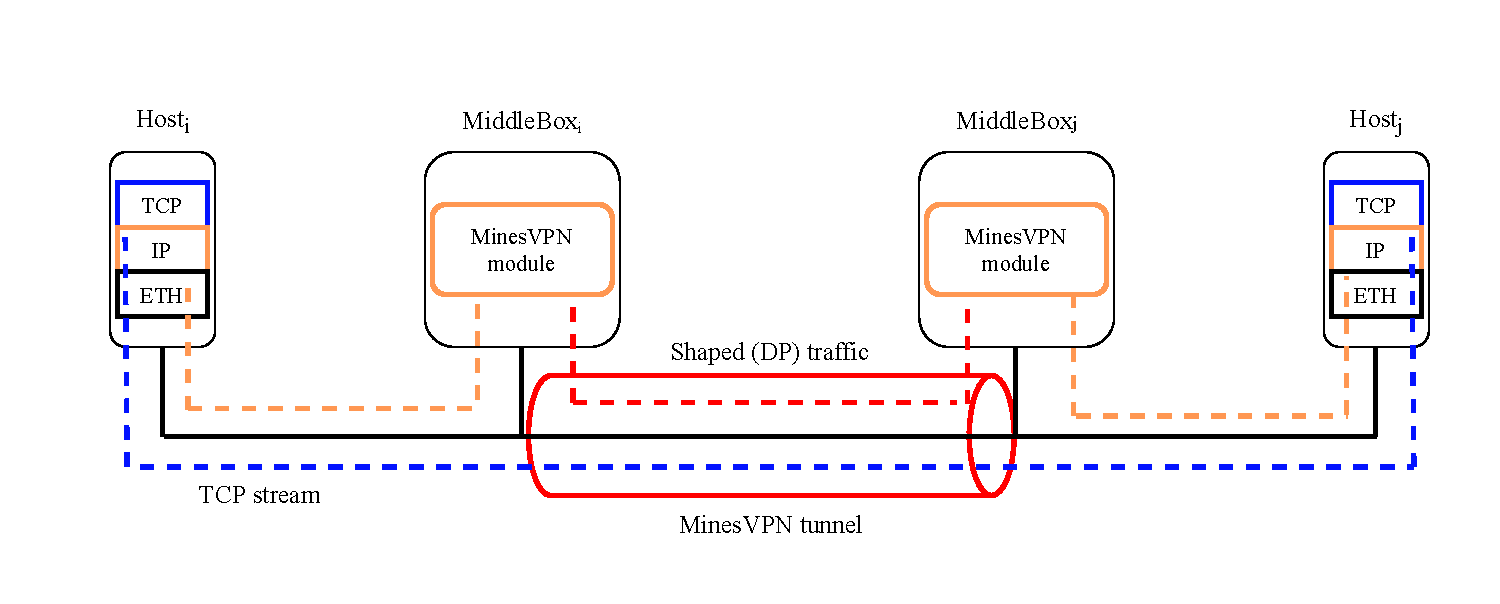
\includegraphics[width=\columnwidth]{figures/Design_highlevel.pdf}
  %  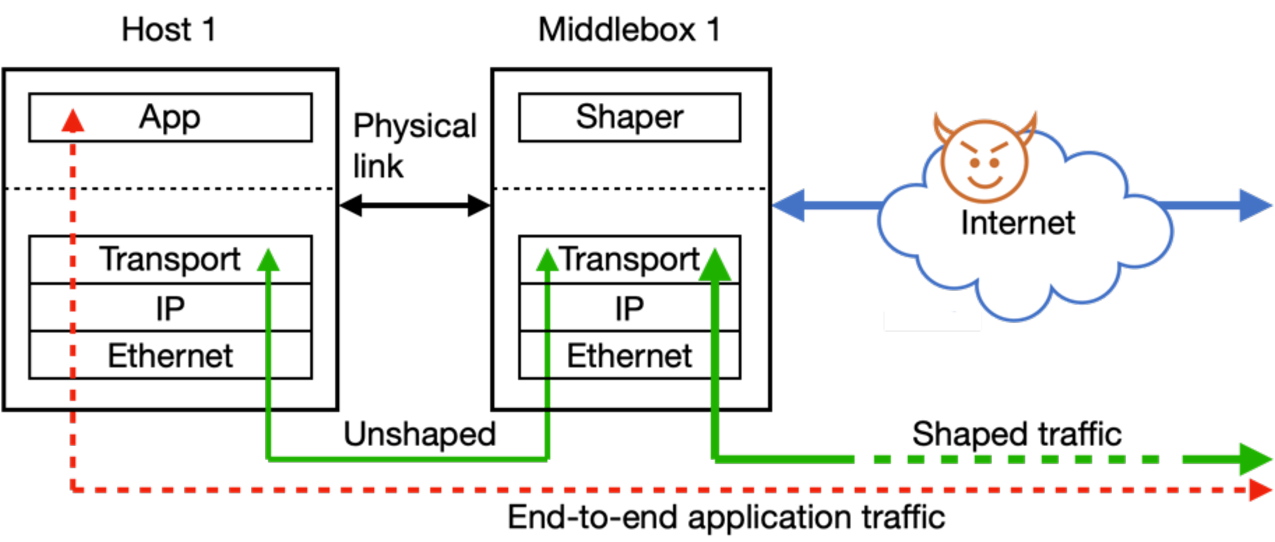
\includegraphics[width=\columnwidth]{figures/minesvpn-overview-half.pdf}
  %  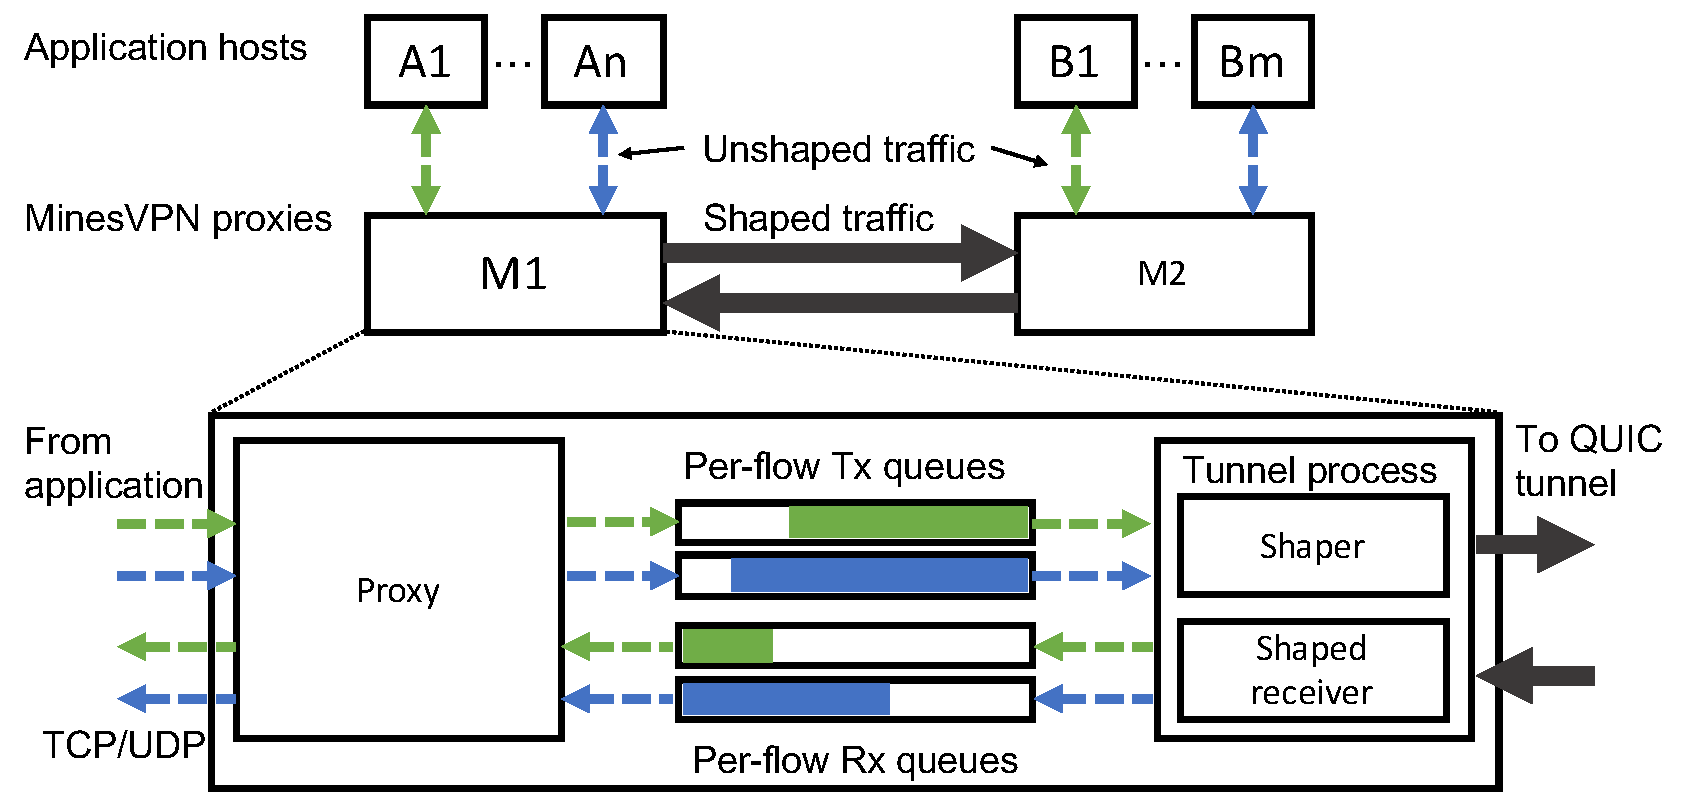
\includegraphics[width=\columnwidth]{figures/minesvpn-arch4.pdf}
  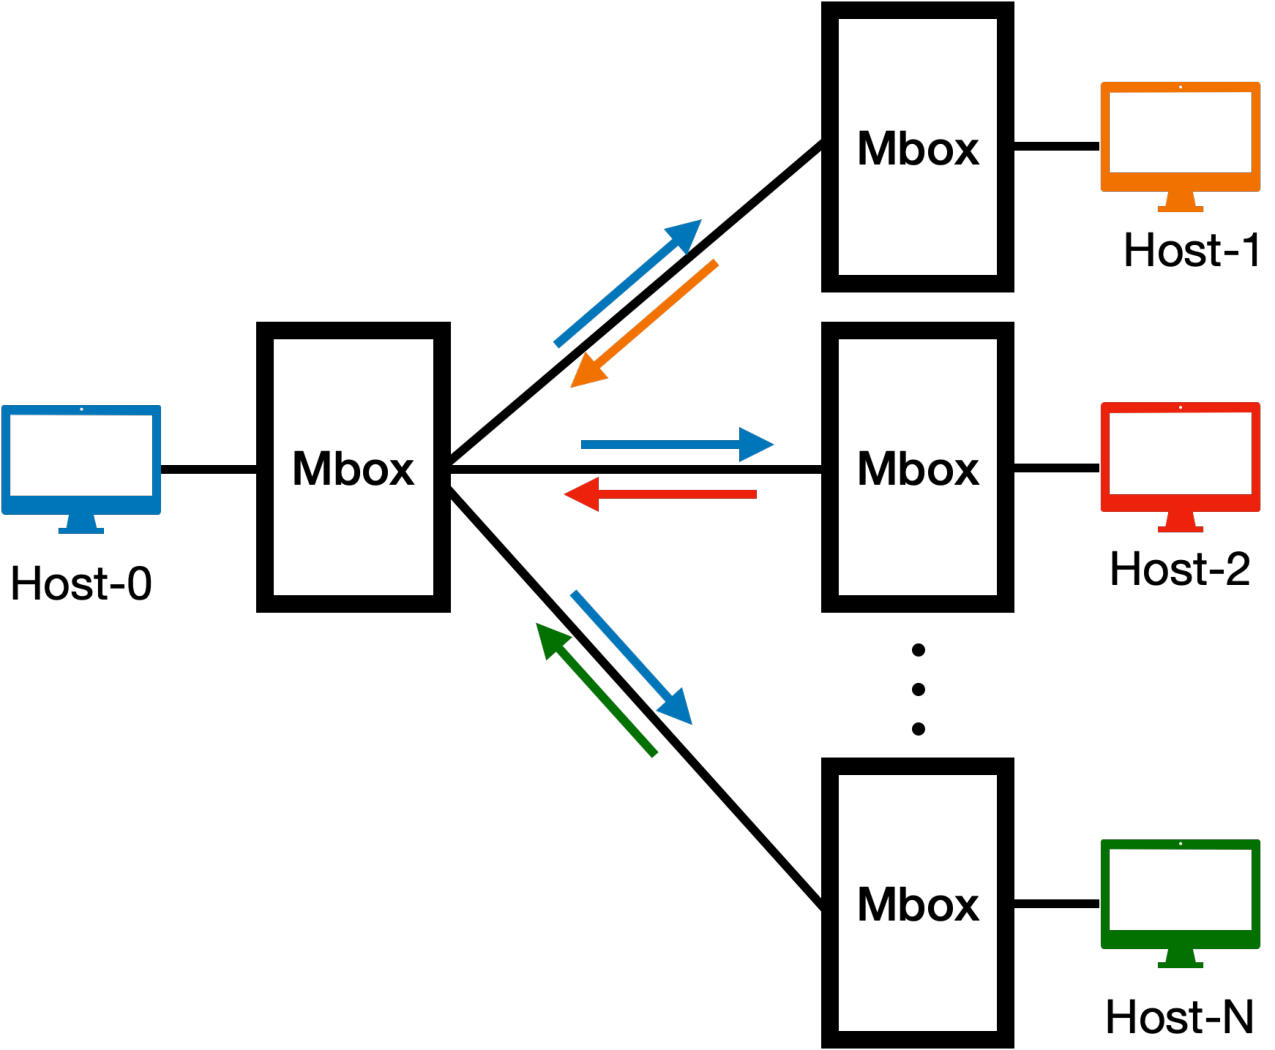
\includegraphics[width=0.7\columnwidth]{figures/one-to-many-communication.pdf}
  \caption{
    One-to-Many parallel communication.
  }
  \label{fig:one-to-many-communication}
\end{figure}



We extend the concept of \textit{buffering queue} that we introduce in \Cref{sec:dp-shaping-definitions} to a \textit{set of $N$ buffering queues} for an application, one for each of pair of communicating parties.  
Each of these queues enqueue the incoming data from application parallel streams with one party within windows of the size of $W$. 
In other words, \Cref{assumption:window} holds true for all $N$ queues simultaneously. 
Similar to \Cref{sec:dp-shaping-definitions}, we define a set of stream subsequences over a window $j$ and represent it with $\istream_j = <\istream^1_j, \istream^2_j, \dots, \istream^N_j>$, such that $k \in [N]:~\istream_j^k = \{P^{\istream^k}_i | P^{\istream^k}_i \in \istream^k~and~t_i^{S^k} \in j\}$. 
Intuitively, a set of stream subsequences is a slice with a length $W$ across all parallel communications with $N$ parties.
We re-define the \Cref{def:neighboring-streams} to match the new setup.
\begin{definition}[Neighboring Series of Streams]\label{def:neighboring-series-stream}
  Two sets of $N$ stream subsequences $S_{j}$ and $\hat{S}_{j}$ transmitted in a window $j$ are neighbors if the L1-norm distance between all corresponding subsequences is at most~$\ssens$ bytes in a window of up to length $\winlen$.
  \\
  In other words: 
  \begin{equation*}
    \forall k \in [n]: {\norm{~S_{j}^k - \hat{S}_{j}^k~}}_1 \leq \ssens
  \end{equation*}
\end{definition}
\noindent
For each subsequence, we define the sensitivity value of its dedicated queue over the intervals of length $T$. 
We represent the sensitivity of a subsequence $S_{j}^k$ with $\qsens^k$: 
\begin{equation}
  \qsens^k = \max_{l = 0}^{\numupdates}~\max_{\streamw{j}^k,
      \hat{\streamw{j}^k}} | \qlent{l}^k - \hat{\qlent{l}^k} |
  \label{eqn:ssens-multi-stream}
\end{equation}
where $\qlent{l}^k$ and  $\hat{\qlent{l}^k}$ are queue lengths of the subsequence $S_{j}^k$ and subsequence $\hat{S_{j}^k}$ at the beginning of the $l$\textsuperscript{th} interval respectively.
The shaping mechanism is independently applied to each packet subsequence, $S_{j}^k$, at intervals of $T$ based on its sensitivity, $\qsens^k$, as we explained in \Cref{subsec:dp-shaping-mechanism}.
Therefore, each queue measurement is $(\varepsilon_T, \delta_T)$-DP.
The transmitted packet sequence is denoted as $N$ sequences of packets observable by adversary:
\begin{equation}
  \ostream = <\ostream^1, \ostream^2, \dots, \ostream^N>
\end{equation}
\noindent 
where we have:
\begin{align*}
  \ostream^1 &= \{{P^{O^1}_1}, {P^{O^1}_2}, {P^{O^1}_3}, \dots \} \\
  \ostream^2 &= \{{P^{O^2}_1}, {P^{O^2}_2}, {P^{O^2}_3}, \dots \} \\
  \vdots& \\
  \ostream^N &= \{{P^{O^N}_1}, {P^{O^N}_2}, {P^{O^N}_3}, \dots \} 
\end{align*} 
We assume that the adversary's goal is to expose the contents of a single packet sequence, $\ostream^k$.
In pursuit of this objective, the adversary strategically exploits the information made available through other packet sequences.
To calculate the privacy loss of measuring all queues for all stream subsequences at each interval, we need to differentiate between two different communication setup: Independent subsequences and Correlated subsequences.   

To measure dependency between stream subsequence, we use the correlation between two streams such that for an application stream with $N$ series of packet sequences $\istream = <\istream^1, \istream^2, \dots, \istream^N>$, we have:
\begin{equation*}
  \forall i,j \in [N]:~Corr(\istream^i, \istream^j) = c_{ij}
\end{equation*}
\noindent
This enables us to define a correlation matrix $C$ such that $[C]_{ij}=c_{ij}$.
We assume the correlation coefficients to have the following properties:
\begin{enumerate}
  \item For all $i,j \in [N]$, $-1 \leq c_{ij} \leq 1$, with $-1$ representing that two subsequences are negatively correlated (\ie when one exists in the stream the other one does not and vice versa), $1$ representing that they are fully correlated (\ie they appear in the stream always together), and $0$ means no correlation.
  \item For all $i \in [N]$, $c_{ii} = 1$.
\end{enumerate}
Various correlation metrics fulfill the aforementioned conditions, with the Pearson correlation coefficient~\cite{cohen2009pearson} being the most prevalent among them. 
\noindent
Calculating privacy loss for independent sequences (\ie $\forall i \neq j \in [N]:~corr(\istream^i, \istream^j) = 0$) is straightforward. 
In independent communication setup, monitoring one sequence does not reveal any information about others. 
Therefore, each stream subsequence is $(\varepsilon_T, \delta_T)$-differentially private.
Nonetheless, in a correlated setup, the adversary has the ability to monitor a single stream, thereby acquiring preceding information about others, which consequently results in further privacy breaches. 
In the following section, we present a systematic approach for quantifying privacy loss in interdependent stream subsequences.
















% \subsection{One-to-Many Independent Communication}
% In this regime of communication, We assume an application is communicating with $N$ parties independently.
% If we represent an application stream with $N$ series of packet sequences $\istream = <\istream^1, \istream^2, \dots, \istream^N>$, all packet sequences are mutually uncorrelated:
% \begin{equation*}
%   \forall i \neq j \in [N]:~corr(\istream^i, \istream^j) = 0
% \end{equation*}
% \noindent
% This assumption is particularly correct for message passing and video streaming applications as these applications provide service for non-related entities.
% For this setup, we argue that the privacy loss of measuring all subsequence queues with DP is the same as privacy loss associated with each individual queue.
% \begin{proposition}\label{prop:independent-subsequence}
%   Assume all packet sequences within an application stream are mutually uncorrelated, if we measure each subsequence queue size with $(\varepsilon_T, \delta_T)$-DP with a sensitivity of $\qsens^k$, measuring queue sizes for all subsequences is also $(\varepsilon_T, \delta_T)$-DP.  
% \end{proposition} 
% \begin{proof}
%   (informal) As packet subsequences are independent, releasing a DP measurement of a queue for one subsequence does not affect the adversary's prior knowledge regarding any other subsequences. 
%   Therefore, the privacy loss associated with the communication between a single pair does not change. 
% \end{proof}
% \noindent
% Based on \Cref{prop:independent-subsequence}, we can measure the privacy loss of a 1-to-$N$ communication simply by extending results of \Cref{prop:dp} to a multiparty communication as follows:
% \begin{proposition}\label{prop:independent-stream-privacy}
%   In the one-to-many independent communication setup, {$\sys$} enforces $(\varepsilon_{\winlen}, \delta_{\winlen})$-DP for each pair of communicating entities within the window of length $W$, with $\varepsilon_{\winlen}, \delta_{\winlen} \triangleq
%   \textrm{DP\_compose}(\varepsilon_T, \delta_T, \numupdates)$.
% \end{proposition}


\subsection{One-to-Many Correlated Communication}
In many applications,  simultaneous communications with distinct entities are interdependent.
For example, many businesses use online advertising platforms such as Google Ads to create and run ads on various websites.
Therefore, every time a user requests the website, the web browser retrieves content from both the web server hosting the website and the online advertising platform that hosts the website's Ads.   
This is, in fact, an example of a one-to-many correlated communication setup.
\\
In standard definition of differential privacy, we assume data points to be independent.  
However, measuring the privacy loss when entries of database are correlated is challenging.
We use two different approaches to tackle this problem. 
\subsubsection{Adjusting Sensitivity for Correlated Communication}


\subsubsection{Composition of Privacy Loss for Correlated Communication}


One approach to ensure DP guarantees for a correlated communication involves multiplying the sensitivity of each packet sequence by the number of correlated packet sequences (\ie $((\qsens^k)_{corr}) = N.\qsens^k$).
Chen\etalc{chen2014correlated} prove this approach to be differentially private.
However, this method implicitly assumes that all correlated sequences are fully correlated, leading to excessive overhead.
To avoid this assumption, we use correlated differential privacy setup proposed by Zhu\etalc{zhu2014correlated} to calculate the privacy loss of our shaping mechanism in one-to-many correlated communication regime.

Following the approach of Zhu~\etal, for each packet sequence, we define correlated sensitivity for each packet sequence:
\begin{definition}[Correlated Sensitivity]\label{def:correlated-sensitivity} 
  For each packet subsequence $S_{j}^k$, we define the correlated sensitivity value of its dedicated queue over the interval of length of $T$, and calculate it as follows:
  \begin{equation}\label{equ:correlated-sensitivity}
    (\qsens^k)_{corr} = \sum_{m=0}^{N} |c_{mi}|. \big( \max_{l = 0}^{\numupdates}~\max_{\streamw{j}^m,
    \hat{\streamw{j}^m}} | \qlent{l}^k - \hat{\qlent{l}^k} | \big) 
  \end{equation}
\end{definition}
\noindent Intuitively, the correlated sensitivity for a packet sequence captures the effect of adding/removing all other packet sequences on the designated sequence.
From \Cref{def:correlated-sensitivity}, it is clear that:
\begin{equation*}
  \qsens^k \leq (\qsens^k)_{corr} \leq N.\qsens^k
\end{equation*} 
\noindent
With \Cref{def:correlated-sensitivity}, we can re-state \Cref{prop:independent-subsequence} for correlated packet sequences.
\begin{proposition}\label{prop:dependent-subsequence}
  Assume there is correlation between packet subsequences of an application stream, if we measure each subsequence queue size with $(\varepsilon_T, \delta_T)$-DP with a sensitivity of $(\qsens^k)_{corr}$ (see \ref{equ:correlated-sensitivity}), measuring queue sizes for all subsequences is also $(\varepsilon_T, \delta_T)$-DP.  
\end{proposition}
\begin{proof}
  Zhu\etalc{zhu2014correlated} prove that if we scale the noise of a randomized differentially private randomized mechanism with adjusted the sensitivity of \Cref{equ:correlated-sensitivity}, it provides DP. The privacy of our mechanism naturally derives from this statement. 
\end{proof}
\noindent Similarly, \Cref{prop:independent-stream-privacy} holds true for interdependent packet sequences within an application stream. 
\begin{proposition}\label{prop:dependent-stream-privacy}
  In the one-to-many correlated communication setup, {$\sys$} enforces $(\varepsilon_{\winlen}, \delta_{\winlen})$-DP for each pair of communicating entities within the window of length $W$, with $\varepsilon_{\winlen}, \delta_{\winlen} \triangleq
  \textrm{DP\_compose}(\varepsilon_T, \delta_T, \numupdates)$.
\end{proposition}



\backmatter
%    7. Index
% See the makeindex package: the following page provides a quick overview
% <http://www.image.ufl.edu/help/latex/latex_indexes.shtml>


\end{document}
